\documentclass{article}
%% to use a package, just delete the % character to enable the package in this document, only on the lines where there is a single % character (otherwise it won't compile)
%% to understand the utility of the package, please read the comment between \begin{comment} and \end{comment} right below the package you need
\usepackage[a4paper, total={6in, 8in}]{geometry} % for european user

%% for multiple lines comment in LaTeX
\usepackage{verbatim} % (won't compile if this line is deleted)
%% usage :
\begin{comment}
	Your multiple lines comment
\end{comment}


%% to include images
\usepackage{graphicx}
\graphicspath{ {./Pictures/} }
\usepackage{float}
%% usage :
\begin{comment}
	\begin{figure}
		\centering (not necessary but it's prettier)
		\includegraphics[scale=(1 by default)]{path to the image/imageName.extension}
		\if you want to put another image side to side, just add a line like the previous
		\caption{picture(s) in a nutshell} (not necessary but it's useful) (won't compile if missing)
	\end{figure}
\end{comment}


%% pour insérer des liens
\usepackage{hyperref}
%% usage :
\begin{comment}
	\href{the complete link}{the display text}
	or if you want to show the complete link, just use 
	\url{the complete link}
\end{comment}


%% to display code easily (insert --shell-escape option when compile, otherwise, it won't compile)
%\usepackage{mint}
%% usage :
\begin{comment}
	- first, you have to have python3-pygments installed on your computer
	\begin{minted}{<language you choose>
		Your code
	\end{minted}
\end{comment}

%% to display code (for more informations, please see : https://texdoc.org/serve/listings.pdf/0)
%\usepackage{listings} 
%% usage :
\begin{comment}
	- listings package let you highly customize how you code will be displayed on the document
	- for simple display just do this :
	\lstdefinestyle{mystyle}{
		Your customizations
	}
	\begin{lstlisting}[language=<the language you'll use)
		Your code
	\end{lstlisting}
\end{comment}

%% to use maths and other sciences symbols (cf https://www.cmor-faculty.rice.edu/~heinken/latex/symbols.pdf) (
%\usepackage{amssymb,amsmath,amsfonts,extarrows}
%% usage : just type the backslash chararacter and the name of the symbol you want, depending of document on the the previous link

%% Have to find the goal of it
%\usepackage{soul}
%\let\oldemptyset\emptyset
%\usepackage[T1]{fontenc}

%% won't compile if at least one of these three next line is deleted
%% but you can add nothing between the brackets to leave it blank
\author{Amnézic}
\date{}
\title{IT Project Management}

\begin{document}
\maketitle
\newpage
%% not necessary
%% compile twice the first time to display table of content
\tableofcontents
\newpage

\section{Introduction}

\subsection{Definition of a project :}
\textbf{Definition :}
\begin{quote}
	The endeavor undertaken to satisfy a corporate need or objective : temporary work with start and end that deliver a product to a client and that respect scopes.
\end{quote}

The three most important constraints of a project, coming from ressources and quality are:
\begin{itemize}
	\item cost
	\item time : it could not be an on-going process
	\item scope : the product we need to deliver and all the interrelated workpackages undertaken to produce a product
\end{itemize}
If one of these three is modified, the two others are directly impacted. \newline

\subsection{Why does a project success or fail ?}
Beside the fact that a project success depends on the respect of the three main constraints, the success of a project depends of mostly these three "events" ($\geq$50\%):
\begin{enumerate}
    \item user involvement (if the project is finally used)
    \item executive management support (sufficient financial support)
    \item clear statement of requirements
\end{enumerate}

Failed projects are usually due to lack of user input or incomplete/changing requirements. So it's very important to precise what are all the why, what, when and how of the project. \textbf{A project is a success only if the project deliver a benefit to the client, even all the three conditions have been complete.}

\subsection{Advantages of project management :}
Organize well a project isn't so easy but it can increase the guarantee (without ensure it) of the succcess of a project, to be aware of all the constraints and the required ressources like tools, ressources or quality. Do a good project management for one project can help for the future ones by keeping ideas that made the project successful or in the other case, understand why it failed and how fix that for the next one.


\newpage
\section{Planning a project}
Some essential things to consider when beginning a project :
\begin{enumerate}
    \item background
    \item stakeholders
    \item scope
    \item deliverables
    \item project assumptions
    \item methodology
    \item WBS
\end{enumerate}

\section{The background}
The background is a tiny summary of the background of the company that is going to build the project, why it will make the project and why it is the best company to make it. It never takes more than one-side sheet and usually is developped on two paragraphs.

\section{The stakeholders}
\textbf{Definition}
\begin{quote}
	Stakeholders are the people involved in or affected by project activities. To lead the participants in a project effectively, you must understand who the stakeholders are and what their attitudes are toward the project.
\end{quote}


There are two types of stakeholders :

\subsection{Internal :}
The internal stakeholders are people who are directly involved in the project
\begin{itemize}
	\item Owners : 
	\item Users : people who is responsible for the day-to-day details and decisions to the project
	\item Project sponsor : guardian of the business vision, negotiator, communication link to executive management
	\item Team members : responsible for day to day delivery of tasks and has input into the solution
	\item Project manager : primary contact between the firm and the clients and is responsible for the deliverables, human resources and project success
	\item Team leader : responsible for a group team members within a specialized area and responsible for ensuring deliverables are me
\end{itemize}

\subsection{External :}
The external stakeholders are people are not involved in the project at all, however, indirectly could affect the projects outcome.
\begin{itemize}
	\item Labor unions
	\item Government
	\item External customers
	\item Financial institutions
	\item Consumer groups
	\item Special interest groups
	\item Suppliers
\end{itemize}


\section{Scope}
The project's scope is the combination of all project goals and tasks, and the work required to accomplish them. The scope answers to these questions :
\begin{itemize}
	\item What marks the end of the project? 
	\item What lies within the scope of the project?
	\item What definitely does not lie within the scope?
	\item What are the project quality measures? 
	\item What is NOT in scope ?
\end{itemize}

\begin{figure}[H]
	\centering
	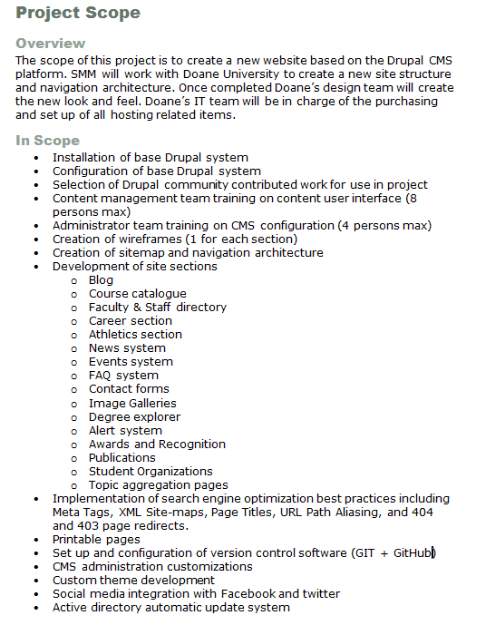
\includegraphics[scale=0.3]{Scope1.png}
	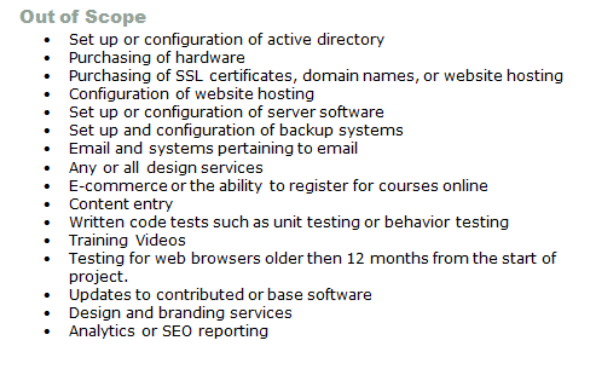
\includegraphics[scale=0.3]{!Scope1.png}
	\caption{In scope and Not in scope}
\end{figure}


\section{Deliverables :}
\textbf{Deliverables}
\begin{quote}
Deliverables is a list, with a brief description, of everything tangible that the project will produce and have an agreed upon grade and quality that set appropriate expectations for its completion.
\end{quote}

Tangible : mesurable


\begin{quote}
\textit{A deliverable is an element of output within the scope of a project. It is the result of objective-focused work completed within the project process. They can be internal or external.}\newline
For more details, please check \href{https://www.wrike.com/project-management-guide/faq/what-is-a-deliverable-in-project-management/}{What is a deliverable in project management?}
\end{quote}

\section{Project assumptions :}
Assumptions in project management are essentially conditions or factors considered to be true, real, or certain without proof or demonstration. They serve as foundational beliefs upon which project plans and decisions are based. These assumptions often involve aspects like resource availability, stakeholder behavior, external dependencies, and environmental factors. Identifying, documenting, and validating assumptions is crucial for managing risks and ensuring the success of a project.

If you don’t identify assumptions and they happen to occur  the project will suffer, and, conversely, if there are assumptions you identify, the project will usually benefit.

Assumptions could concern :
\begin{itemize}
	\item resources
	\item deliverables
	\item environmental
	\item budgetary
	\item functionality
\end{itemize}

\section{Methodology :}



\section{The WBS}
The Work Breakdown Structure is the process that breaks down an activity into smaller chunks, and this recursively until the activities are "small enough".

The WBS is based on the task dependencies types :
\begin{figure}[H]
	\centering
	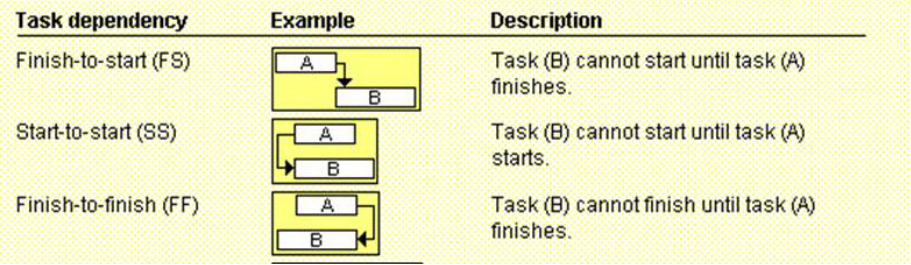
\includegraphics[scale=0.3]{TaskDependency.png}
	\caption{}
\end{figure}

Tasks can be with a lead or a lag time :
\begin{itemize}
	\item lead : a task B that has to be begin during the task A process (negative lag time value)
	\item lag : a task B that can't be begin before task A is finished. B task can be begin at the exact end of the task A or after the end of task A (positive lag time value)
\end{itemize}

To prepare a WBS, we have to follow these steps :
\begin{enumerate}
	\item identify the major sets of activities
	\item break the major activities down further
	\item allocate duration to the tasks
	\item determine the dependencies between the activities
\end{enumerate}

\section{Cost management}
\subsection{Resource planning}

\subsection{Cost estimating}
They are different ways to estimate a budget :
\begin{itemize}
	\item detail/bottom up estimation : estimate based on the detailed tasks of a complex project (+++ time consuming) (target range from -5\% to +10\%)
	\item historical estimate : estimation based on the actual budget of previous project (from -15\% to +25\%)
\end{itemize}


Principles for estimating 
\begin{itemize}
	\item base the estimates on the performance of average staff
	\item estimates has to be done and reviewed by qualified people
	\item reflect the most likely cost and not a padded one
	\item allowance needs to be made for :
	\begin{itemize}
		\item contingencies
		\item high risks (from assumptions)
		\item scope changes
		\item unknowns
	\end{itemize} 
\end{itemize}


\textbf{Challenges of estimating}\newline
Cost estimations are a complex tasks that requires a significant amount of effort, and people have a bias towards underestimation that can be curves by learning how to do estimations.\newline

Don't estimate well the cost of a project could be very harmful for the project. Bad estimation could come from :
\begin{itemize}
	\item price escalation
	\item exchange rates
	\item requirements unclear
	\item scoop creep
	\item technical complexity
	\item historical data ($\neq$ from historical cost estimation : historical data it's just all the type of data that we reuse from a previous project to the current project)
	\item integration
	\item new technology
	\item external dependencies
\end{itemize}

\subsection{Cost budgeting}
Project budget consists of direct costs (staff charges, expenses), indirect costs (all the is not directly linked to the project but that is required for the project (paper towels for example)) and capital costs (equipment, servers ...).\newline
\newline

It's possible to alter the budget by :
\begin{itemize}
	\item staff rates
	\item expenses
	\item capital costs : negotiate the best prices and amortize the equipment
\end{itemize}



\subsection{Cost control}
\subsection{Change control}

\section{Risk}
Mitigate the risk : respond to the risk
risk : something that could go wrong
\newline
Risk identification process
\subsection{Risk identification}
A good rule of thumb is to identify risks using logical categories (like technical, business, legal, natural events etc...).\newline

Examples of risks events :
\begin{itemize}
	\item scope creep
	\item server downtime
	\item server purchasing delays
	\item no cooperation from departments or users
\end{itemize}



\subsection{Risk quantification}
The level of a risk in a project is determined by :
\begin{itemize}
	\item probability
	\item impact if occured
	\item category of the risk
\end{itemize}

\begin{figure}[h]
	\centering
	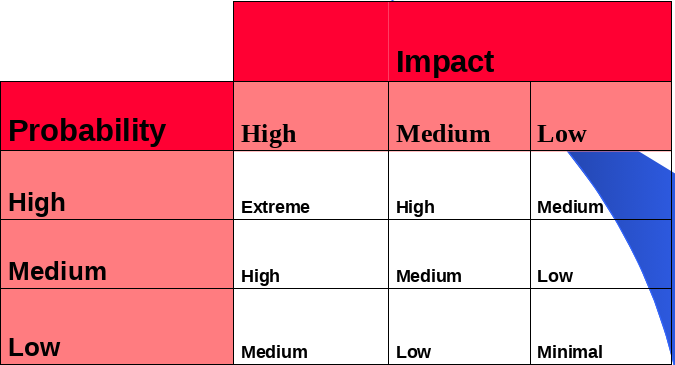
\includegraphics[scale=0.5]{riskLevel.png}
	\caption{Risks levels sum up}
\end{figure}





\subsection{Risk response development}
\subsection{Risk response control}

\end{document}
